\chapter{Implementation}

This chapter focus on the implementation details of two add-ons:
\begin{enumerate}
\item a malicious add-on, which can infect the victim`s filesystem
\item a Transcriptase detection add-on, which can detect the metamorphic malware embedded in the web page.
\end{enumerate}

\section{Malicious add-on}

Generally browsers like Firefox, Chrome, and Opera do not allow access to the client filesystem using JavaScript. Even though creating a file is possible in IE using ActiveX objects, the client must enable ActiveX scripts on their system for the ActiveX object related code to execute properly [36]. 

Firefox add-ons are very powerful because of the high-level APIs that the SDK provides. The SDK has a file I/O module which provides access to the client`s filesystem.

A malicious add-on was created to demonstrate the way that a victim`s machine may get infected by a malicious add-on. The basic functionality of this add-on is it provides the statistic value i.e., the total JavaScript bytes in the page loaded by the user as shown in the Figure ~\ref{fig:maliciousaddon}.

\begin{figure}
    \centering    
    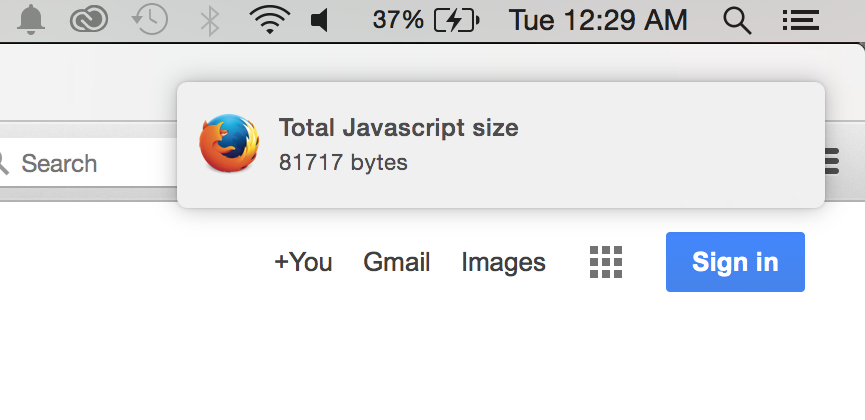
\includegraphics[width=8cm, height=3.9cm]{maliciousaddon.png}
    \caption[Main Functionality of the malicious add-on]{Main Functionality of the malicious add-on}
    \label{fig:maliciousaddon}
\end{figure}

The user expects this functionality and installs the malicious add-on, but this add-on also has hidden functionality. Whenever it finds that web page content has Transcriptase in it, it finds all the JavaScript files present in the filesystem and prepends them with Transcriptase code and thus it infects the victim`s filesystem. 

\begin{figure}
    \centering    
    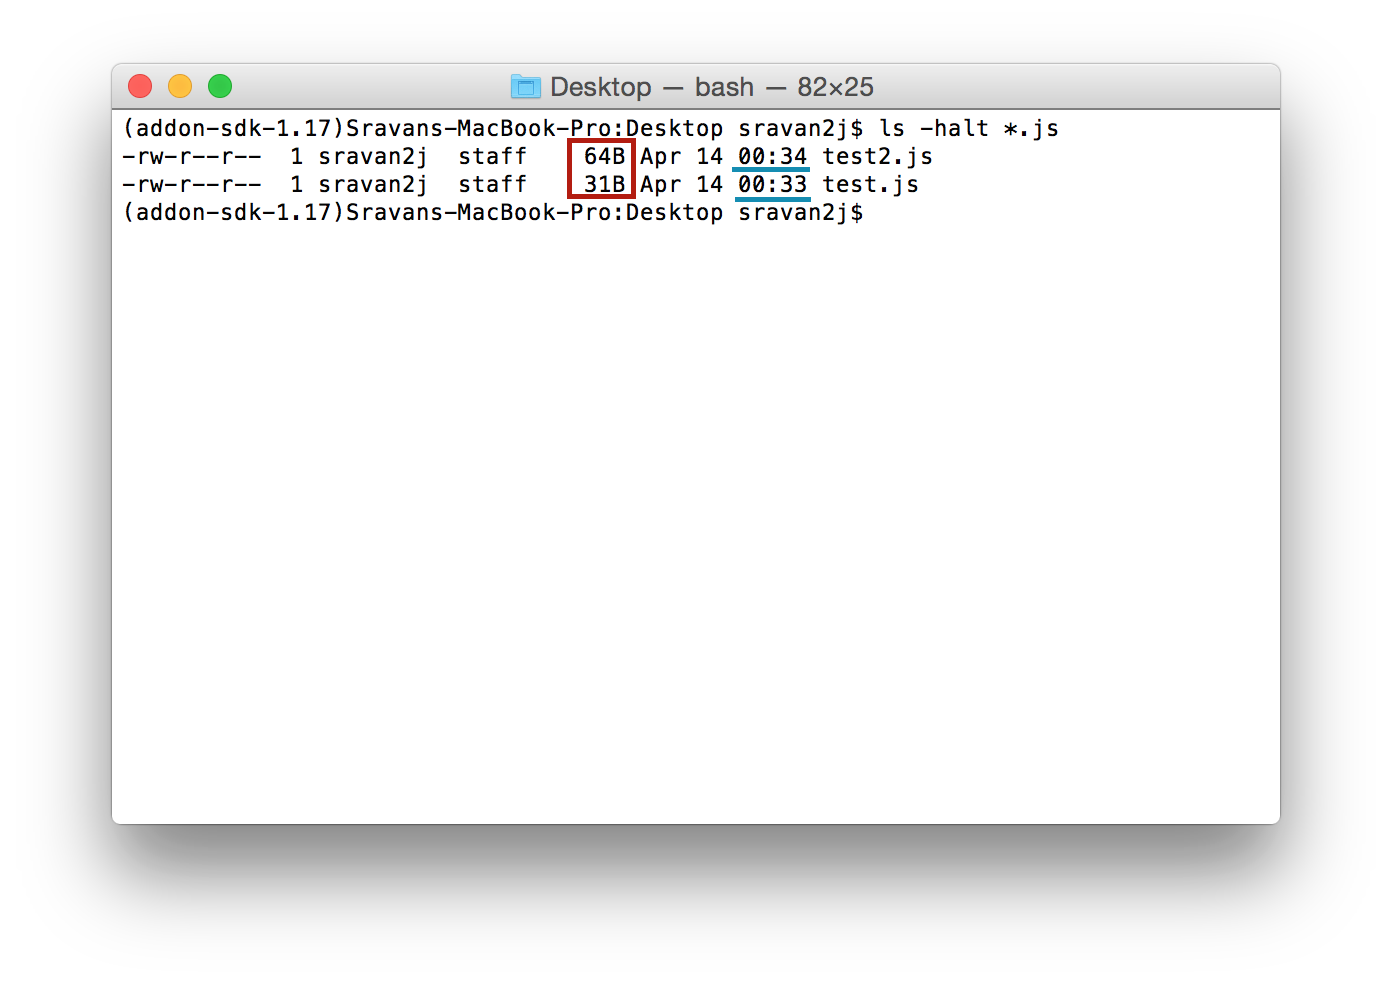
\includegraphics[width=17cm, height=11.95cm]{beforeinf.png}
    \caption[Size of sample JavaScript files before infection, ]{Size of sample JavaScript files before infection}
    \label{fig:beforeinf}
\end{figure}
\begin{figure}
    \centering    
    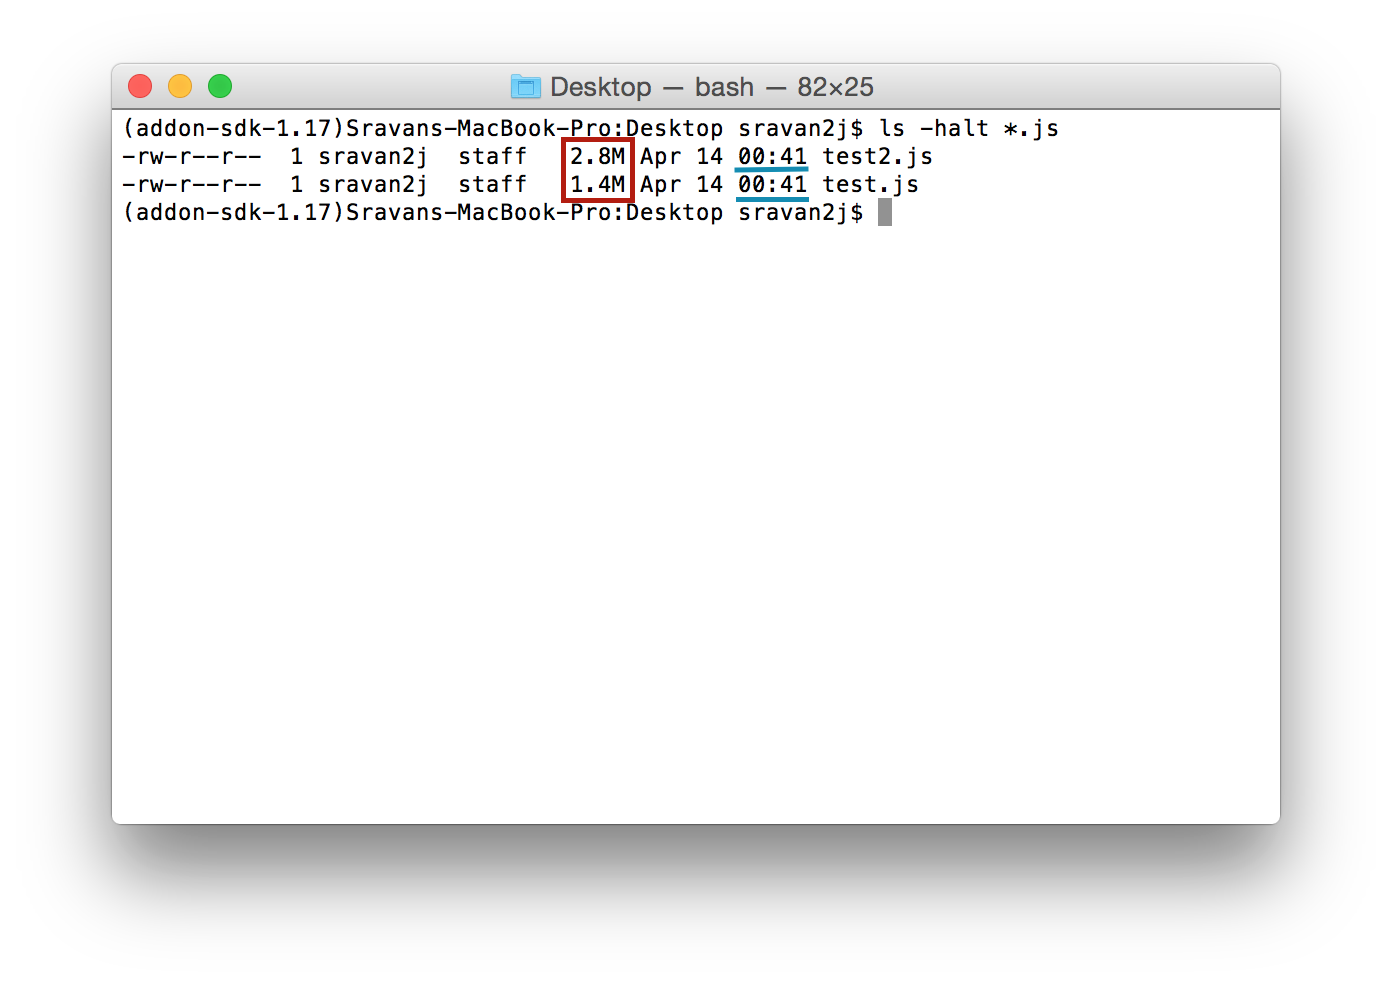
\includegraphics[width=17cm, height=11.95cm]{afterinf.png}
    \caption[JavaScript file sizes after infection]{JavaScript file sizes after infection}
    \label{fig:afterinf}
\end{figure}

Figure~\ref{fig:beforeinf} shows the size of our sample JavaScript files before infection and figure~\ref{fig:afterinf} shows the size of these files after infection. There is a huge difference in file sizes before and after infection. This infection will remain unknown to the user until the infected files are checked.

\section{Transcriptase detection add-on} 

As discussed in Section \ref{transcriptasesection}, Transcriptase virus uses different techniques to change its internal structure in order to evade the signature based detection strategy. Transcriptase detection add-on can detect the Transcriptase malware included in the webpage and notifies the user about the presence of malware without loading the JavaScript malware.

\subsection{Malware Detection Technique} 
Despite the fact that metamorphic malware continuously changes its internal structure to stay undetected, still for maintaining its functionality malware places similar instructions (that implements the functionality) somewhere in the code. Thus, all the morphed copies maintains same statistical distribution of instructions. Different malware detection strategies are designed to make use of these statistical properties like Hidden Markov Model, Opcode Graph Similarity, Simple Substitution Distance, and Singular Value Decomposition.

As mentioned in [4], if the files are having highly similar opcode statistics, then Opcode Graph Similarity and Singular Value Decomposition can classify them better than the Hidden Markov Model and Simple Substitution Distance. Though, Opcode Graph Similarity and Singular Value Decomposition are very sensitive to deadcode, but from the results mentioned in [4] these strategies won`t be able to distinguish between benign code and virus code only after adding 5000 and 9000 deadcode functions into the virus code respectively. And it is extremely uncommon that a web page having this much of dead code functions. Adding to this, ROC curves in [4] shows that Opcode Graph Similarity performs better than Singular Value Decomposition for the less number of dead code function insertions up to 1000.

We used Opcode Graph Similarity technique in the Transcriptase detection add-on.

\subsection{Opcode Graph Similarity Technique}

In [3], Anderson introduced a malware detection technique which is based on analysis of graphs that are constructed using the opcodes of the malware code and test code. In this technique, initially opcodes are extracted from the malware code and a weighted directed graph is built using the sequence of opcodes. Similarly, a graph is built for the code to be tested. Manhattan distance between these two weighted graphs specifies the test file score [4].

\subsection{Opcode Graph}

A weighted directed graph built using the sequence of opcodes is known as `Opcode Graph'. Each node of this graph specifies a distinct opcode in opcode sequence. A directed edge exists from $node_A$ to $node_B$, if $node_B$`s opcode follows the $node_A$`s opcode in the opcode sequence. Weight of the edge from $node_A$ to $node_B$, specifies the total number of times that the $node_B$`s opcode follows the $node_A$`s opcode in the entire code. 

\begin{figure}[h]
  \centering
\begin{lstlisting}[frame=none,language=myasm,multicols=2] 
PUSH
MOV
SUB
AND
MOV
TEST
JZ
INT
MOVZX
AND
MOV
MOVZX
OR
MOV
MOV
CALL
LEAVE
RETN
ALIGN
PUSH
MOV
MOV
PUSH
PUSH
SUB
MOV
MOV
CALL
AND
SUB
CALL
MOV
CALL
MOV
XOR
MOV
MOV
MOV
CALL
MOV
\end{lstlisting}
    \caption[Sample opcode sequence]{Sample opcode sequence.}
    \label{fig:opcodesequence}
\end{figure}

\begin{figure}[h]
  \centering
\begin{tabular}{c|cccccccccccccc}
  & \begin{sideways}ALIGN\end{sideways}  & \begin{sideways}AND\end{sideways}  & \begin{sideways}CALL\end{sideways}  & \begin{sideways}INT\end{sideways}  & \begin{sideways}JZ\end{sideways}  & \begin{sideways}LEAVE\end{sideways}  & \begin{sideways}MOV\end{sideways}  & \begin{sideways}MOVZX\end{sideways}  & \begin{sideways}OR\end{sideways}  & \begin{sideways}PUSH\end{sideways}  & \begin{sideways}RETN\end{sideways}  & \begin{sideways}SUB\end{sideways}  & \begin{sideways}TEST\end{sideways}  & \begin{sideways}XOR\end{sideways} \\
 \midrule
ALIGN&  0& 0& 0& 0&  0& 0& 0&  0& 0&1& 0&0&  0&0 \\
AND& 0&0&0&0&  0&0& 2&  0& 0&0& 0&1&  0&0 \\
CALL&0&1&0&0&  0&1& 3&  0& 0&0& 0&0&  0&0 \\
INT& 0&0&0&0&  0&0& 0&  1& 0&0& 0&0&  0&0 \\
JZ&  0&0&0&1&  0&0& 0&  0& 0&0& 0&0&  0&0 \\
LEAVE&  0&0&0&0&  0&0& 0&  0& 0&0& 1&0&  0&0 \\
MOV& 0&0&4&0&  0&0& 5&  1& 0&1& 0&1&  1&1 \\
MOVZX&  0&1&0&0&  0&0& 0&  0& 1&0& 0&0&  0&0 \\
OR&  0&0&0&0&  0&0& 1&  0& 0&0& 0&0&  0&0 \\
PUSH& 0&0&0&0&  0&0& 2&  0& 0&1& 0&1&  0&0 \\
RETN&1&0&0&0&  0&0& 0&  0& 0&0& 0&0&  0&0 \\
SUB& 0&1&1&0&  0&0& 1&  0& 0&0& 0&0&  0&0 \\
TEST&0&0&0&0&  1&0& 0&  0& 0&0& 0&0&  0&0 \\
XOR& 0&0&0&0&  0&0& 1&  0& 0&0& 0&0&  0&0 \\
\end{tabular}
    \caption[Weight counts adjacency matrix for opcode sequence]{Weight counts adjacency matrix for opcodes in Figure~\ref{fig:opcodesequence}.}
    \label{fig:weightcounts}
\end{figure}

Figure ~\ref{fig:opcodesequence} shows the sample opcode sequence. Adjacency matrix in Figure ~\ref{fig:weightcounts} specifies the weights of the edges formed between these opcodes. For instance, we can find that intersection entry between CALL row and MOV column has weight value 3, which means there are three occurrences of MOV instruction immediately followed by CALL instruction in the opcode sequence i.e., at line numbers 15, 27, and 32 in Figure ~\ref{fig:opcodesequence}. 

All the weight counts in Figure ~\ref{fig:weightcounts} are converted into probability values by dividing each row entry by the corresponding row sum. Figure ~\ref{fig:probabilitymatrix} shows the weight probabilities for the Figure~\ref{fig:weightcounts}. Each weight probability specifies the probability of occurrence of a particular opcode, immediately after the selected opcode [4]. 

\begin{figure}[h]
  \centering
\begin{tabular}{c|cccccccccccccc}
  & \begin{sideways}ALIGN\end{sideways}  & \begin{sideways}AND\end{sideways}  & \begin{sideways}CALL\end{sideways}  & \begin{sideways}INT\end{sideways}  & \begin{sideways}JZ\end{sideways}  & \begin{sideways}LEAVE\end{sideways}  & \begin{sideways}MOV\end{sideways}  & \begin{sideways}MOVZX\end{sideways}  & \begin{sideways}OR\end{sideways}  & \begin{sideways}PUSH\end{sideways}  & \begin{sideways}RETN\end{sideways}  & \begin{sideways}SUB\end{sideways}  & \begin{sideways}TEST\end{sideways}  & \begin{sideways}XOR\end{sideways} \\
 \midrule
ALIGN&  0&0&0& 0& 0& 0&  0&  0&  0&$^1/_1$& 0& 0& 0& 0 \\
AND& 0&0&0& 0& 0& 0&  $^2/_3$&  0&  0& 0& 0& $^1/_3$& 0& 0 \\
CALL&0&$^1/_5$ & 0& 0& 0&  $^1/_5$& $^3/_5$& 0& 0& 0& 0& 0& 0& 0 \\
INT& 0&0&0& 0& 0& 0& 0& $^1/_1$& 0&  0& 0& 0& 0& 0 \\
JZ&  0&0&0& $^1/_1$& 0& 0& 0&  0&  0&  0&  0&  0&  0&  0 \\
LEAVE&  0&0&0& 0& 0& 0& 0& 0& 0&  0&  $^1/_1$& 0&  0&  0 \\
MOV& 0&0&$^4/_{14}$& 0& 0&  0&  $^5/_{14}$& $^1/_{14}$& 0&  $^1/_{14}$& 0&  $^1/_{14}$&  $^1/_{14}$& $^1/_{14}$\\
MOVZX&  0&$^1/_2$& 0&  0& 0&  0&  0&  0&  $^1/_2$&  0&  0&  0&  0& 0 \\
OR&  0&0&0&  0& 0&  0&  $^1/_1$& 0&  0&  0&  0&  0&  0& 0 \\
PUSH&0&0&0&  0& 0&  0&  $^2/_4$& 0&  0&  $^1/_4$&  0&$^1/_4$& 0&  0 \\
RETN&  $^1/_1$& 0&  0&  0& 0& 0&  0&  0&  0& 0&  0& 0&  0& 0 \\
SUB& 0&$^1/_3$& $^1/_3$& 0&  0&  0& $^1/_3$& 0& 0&  0&  0& 0&  0& 0 \\
TEST&0&0&0&  0& $^1/_1$& 0&  0&  0&  0&  0&  0& 0&  0& 0 \\
XOR& 0&0&0&  0&  0&  0&  $^1/_1$&  0&  0&  0&  0&  0&  0&  0 \\
\end{tabular}
    \caption[Probability matrix for weights adjacency matrix]{Probability matrix for weights adjacency matrix in Figure ~\ref{fig:weightcounts}.}
    \label{fig:probabilitymatrix}
\end{figure}

Figure ~\ref{fig:opcodegraph} shows the opcode graph for the probability matrix in Figure ~\ref{fig:probabilitymatrix} 

\begin{figure}[h]
  \centering
      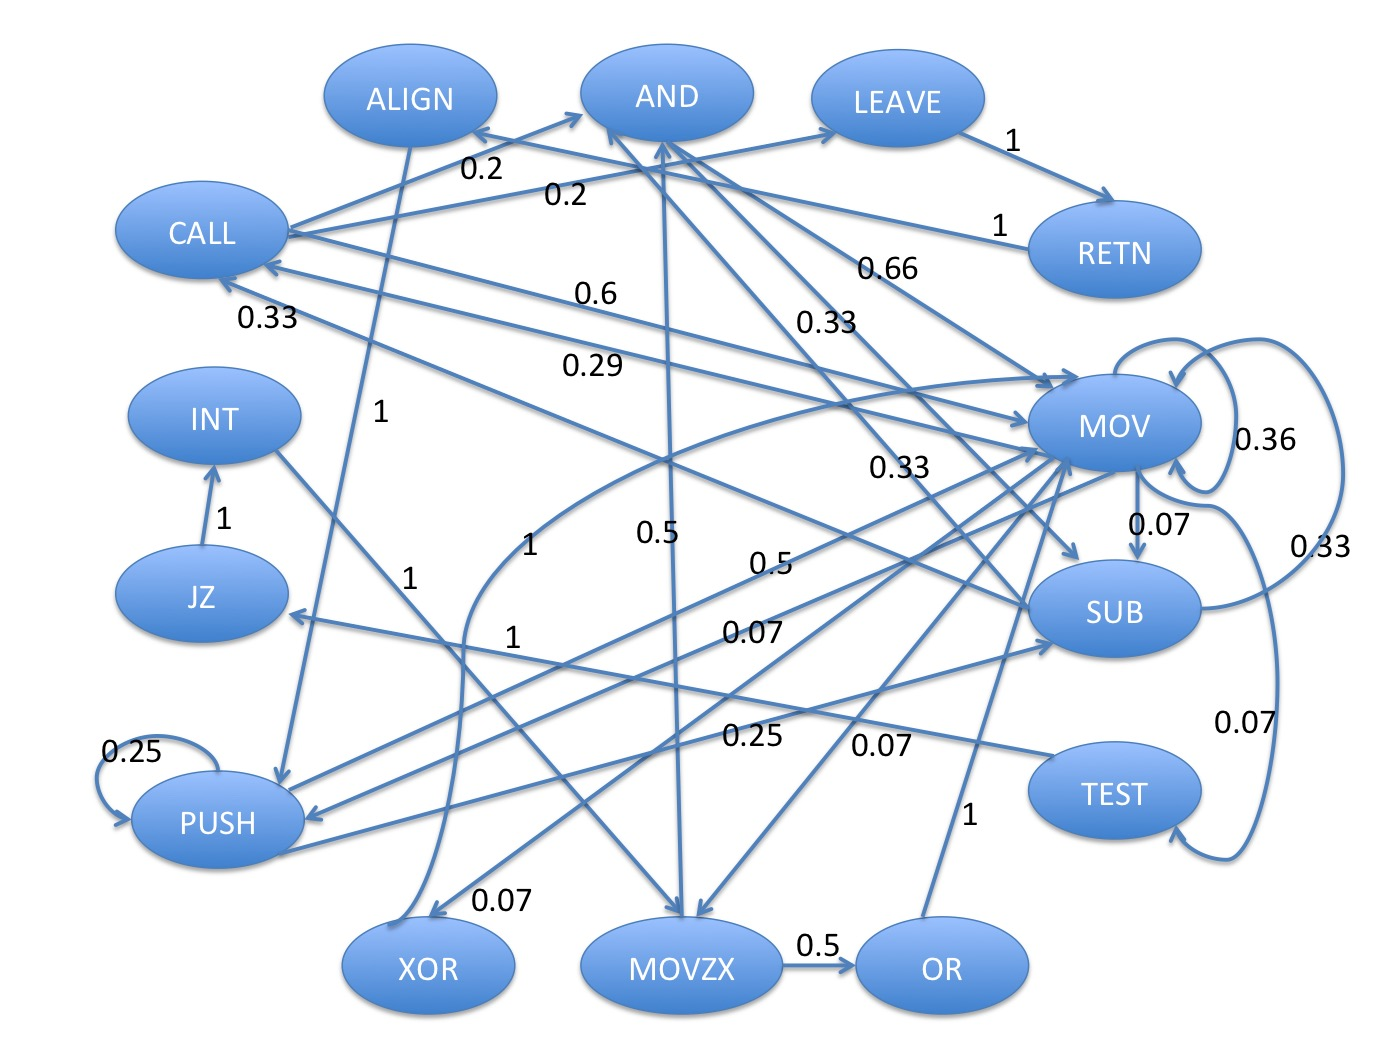
\includegraphics[width=16cm, height=12cm]{opcodegraph.jpg}
    \caption[Opcode Graph]{opcode graph for the probability matrix in Figure [8].}
    \label{fig:opcodegraph}
\end{figure}

\subsection{Similarity Score Calculation}
After creating probability matrices for the malware file and the test file, similarity between two files is calculated by taking the Manhattan distance between two probability matrices. Consider $A$ as the probability matrix of file 1 and each element in $A$ is denoted as $A_i,_j$ where $i$ and $j$ specifies $i^{th}$ row and $j^{th}$ column respectively. Similarly $B$ is the probability matrix of file 2 and each element in $B$ is denoted as $B_i,_j$. Similarity between matrix $A$ and $B$, is calculated as below [8],

Similarity score = ${1 \over N^2}(\sum_{i,j=0}^{N-1}|a_i,_j-b_i,_j|^2)$ 

where N is total number of distinct opcodes present in the combination of both files.

Before using the similarity score, we have to determine the threshold score which distinguishes between benign file and malware file. Threshold value is determined as follows [8],
\begin{enumerate}
\item Construct opcode graphs for all the variants metamorphic malwares.
\item Construct opcode graphs for all the benign files.
\item Calculate the similarity scores for all pairs of malwares.
\item Calculate the similarity scores for every benign files against malware from step 1.
\item Determine a threshold value using the scores calculated in steps 3 and 4.
\end{enumerate}
\textbf{——— BELOW DATA IS JUNK DATA ——–}

	
\LaTeX\ can be viewed
as a compiled programming language, in contrast to that 
nightmare known as Microsoft Word,
which can be viewed as an interpreted language. So, to typeset a
document in \LaTeX, you create a text file that has the {\tt .tex} extension.
This file includes some special
commands, known as macros. Then
you compile your {\tt .tex} file by running  \LaTeX,
which produces your typeset document, as a pdf. 

In this paper, a few basics are discussed. There are plenty of good online resource
if you need help with more advanced topics.


\section{Opcode Graph Similarity} 

To typeset text, you type whatever you want. Multiple spaces are
ignored                           when typesetting, and
the end of a line is treated as another space.
Consequently, when you are typing, you can break lines anywhere, like here
or here,
since the lines are formatted automatically when you typeset the document.
You start a new paragraph by leaving a blank line.

See how easy it is to start a new paragraph? A blank line does the trick.


